Considera la funció
\[
f(x)=x^4-4x^3+4x^2 .
\]

\begin{apartats}

\apartat[1,25]{1}
Troba'n els punts de tall amb els eixos, estudia'n la monotonia i troba'n els extrems
relatius.

\begin{solucio}
\textbf{Talls}: $f(x)=x^2\left(x^2-4x+4\right)=x^2(x-2)^2$. Els talls són $(0,0)$ i $(2,0)$, tots dos
amb arrel doble; $(0,0)$ és també el tall amb l'eix $OY$.\\
\textbf{Monotonia}: $f'(x)=4x^3-12x^2+8x=4x(x-1)(x-2)$, que s'anul·la en $x=0$, $x=1$ i $x=2$.\\
$f$ \textbf{decreix} a $(-\infty,0)$, \textbf{creix} a $(0,1)$, \textbf{decreix} a $(1,2)$ i
\textbf{creix} a $(2,+\infty)$.\\
\textbf{Mínims relatius} $(0,0)$ i $(2,0)$, i \textbf{màxim relatiu} $(1,1)$.
\end{solucio}

\begin{nomesllarg}
\apartat{0,75}
Estudia'n la curvatura i troba'n els punts d'inflexió.

\begin{solucio}
$f''(x)=12x^2-24x+8=4\left(3x^2-6x+2\right)$, que s'anul·la en $x=1\pm\dfrac{\sqrt3}{3}$ (és a dir,
$x\approx0{,}42$ i $x\approx1{,}58$).\\
$f''>0$ fora de l'interval que formen, on la funció és \textbf{convexa}, i $f''<0$ a dins, on és
\textbf{còncava}.\\
Com que la curvatura hi canvia, hi ha dos punts d'inflexió, i tots dos tenen $y=\dfrac49$:
$\left(1-\tfrac{\sqrt3}{3},\tfrac49\right)$ i $\left(1+\tfrac{\sqrt3}{3},\tfrac49\right)$.
\end{solucio}
\end{nomesllarg}

\begin{tria}{estudi-tasca}
\itemtria{original}{0,75}{1,25}
Representa la funció amb tota la informació anterior.

\begin{solucio}
La gràfica baixa fins al mínim $(0,0)$, puja fins al màxim $(1,1)$, torna a baixar fins al mínim
$(2,0)$ i torna a pujar: té forma de W, simètrica respecte de la recta $x=1$. Les dues branques
infinites van cap a $+\infty$.
\begin{center}
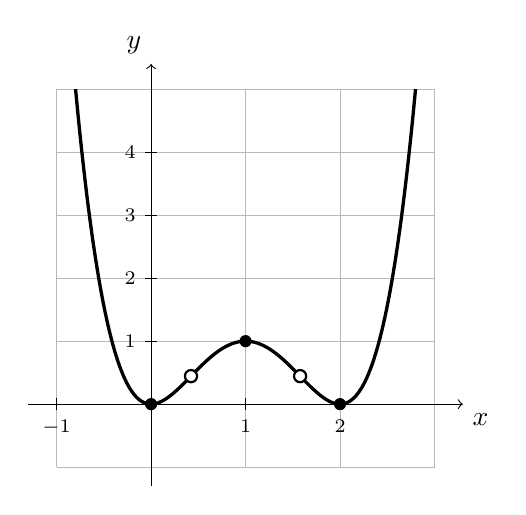
\begin{tikzpicture}[x=1.2cm,y=0.8cm]
  \draw[gray!55,very thin,step=1] (-1,-1) grid (3,5);
  \draw[->] (-1.3,0) -- (3.3,0) node[below right] {$x$};
  \draw[->] (0,-1.3) -- (0,5.4) node[above left] {$y$};
  \foreach \i in {-1,1,2} \draw (\i,0.1) -- (\i,-0.1) node[below,font=\scriptsize] {$\i$};
  \foreach \j in {1,2,3,4} \draw (0.06,\j) -- (-0.06,\j) node[left,font=\scriptsize] {$\j$};
  \begin{scope}
    \clip (-1,-1) rectangle (3,5);
    \draw[\colorgrafica,very thick,domain=-0.8:2.8,samples=150,smooth] plot (\x,{\x*\x*(\x-2)*(\x-2)});
  \end{scope}
  \fill (0,0) circle (2.2pt); \fill (1,1) circle (2.2pt); \fill (2,0) circle (2.2pt);
  \draw[fill=white,thick] (0.4226,0.4444) circle (2.2pt);
  \draw[fill=white,thick] (1.5774,0.4444) circle (2.2pt);
\end{tikzpicture}
\end{center}
\end{solucio}

\itemtria{extrems-absoluts}{0,75}{1,25}
Troba els valors màxim i mínim absoluts de $f$ a l'interval $[-1,3]$, i el recorregut de $f$ a tot
$\mathbb{R}$.

\begin{solucio}
A $[-1,3]$, els candidats són els punts crítics de dins, $x=0$, $x=1$ i $x=2$, i els extrems de
l'interval: $f(0)=0$, $f(1)=1$, $f(2)=0$, $f(-1)=9$ i $f(3)=9$.\\
\textbf{Màxim absolut}: $9$, als dos extrems de l'interval, $x=-1$ i $x=3$. \textbf{Mínim absolut}:
$0$, en $x=0$ i en $x=2$. El màxim relatiu, $(1,1)$, no és l'absolut.\\
A tot $\mathbb{R}$, $f(x)=x^2(x-2)^2\ge0$, el valor $0$ s'assoleix en els mínims, i $f\to+\infty$ pels
dos costats: el recorregut és $[0,+\infty)$.
\end{solucio}
\end{tria}

\end{apartats}
